\chapter{Fundamentação Teórica}

Neste capítulo são apresentados os conceitos relacionados ao desenvolvimento desta pesquisa, bem como o embasamento teórico necessário para o entendimento do estudo. Os temas abordados são: ETL, Banco de Dados NoSQL, Frameworks, Estudo Experimental de Software e trabalhos correlatos ao tema deste trabalho.


\clearpage
% ---

\section{Conceitos Básicos}

Conceitos de ETL, banco de dados NoSQL, \textit{frameworks} e estudo experimental de software são essenciais para esta pesquisa. Dessa forma, os princípios básicos desses conceitos são apresentados nesta seção. Ainda que estudo experimental de software não seja o tema principal deste trabalho, seus conceitos são essenciais para avaliar e medir nossa proposta, sendo assim é fundamental entender seus conceitos.

\subsection{ETL}

ETL sigla para \textit{Extraction, Transform and Load} (Extração, Limpeza/Transformação e Carga) é conhecido na literatura por definir processos que permitem a integração de dados, centralizando-os numa base destino facilitando o gerenciamento e análise dos dados [\cite{kimball:2004}, \cite{rud:2009}]. O fluxo do processo de ETL inicia-se com extração dos dados a partir de uma fonte, que podem ser arquivos textuais, banco de dados relacionais ou banco de dados NoSQL. Os dados são propagados para uma Área de Processamento de Dados onde são executadas a limpeza e transformação por meio de mecanismos de ETL definidos como agregação, junção, filtro, união, entre outros. Finalmente, os dados são carregados em estruturas que podem ser data warehouses ou repositórios analíticos [\cite{silva:2016}]. 

\cite{kimball:2004} definem ETL em quatro macroprocessos, com 34 subsistemas. Os quadros \ref{subextracao}, \ref{sublimpeza}, \ref{subcarga} e \ref{subgerenciamento} mostram os subsistemas do processo de ETL. Os quatro macroprocessos são:

\begin{itemize}
	\item Extração: Recolhe os dados dos sistemas de origem e grava na área de processamento de dados antes de qualquer reestruturação significativa. Esta etapa possui 3 subsistemas.
	
	\item Limpeza e Transformação: Envia os dados de origem, por meio de várias etapas de processamento no sistema ETL. Melhora a qualidade dos dados recebidos da fonte, mescla dados de duas ou mais fontes para criar e aplica dimensões e métricas. Esta etapa possui 5 subsistemas.
	
	\item Entrega ou Carga: Estrutura fisicamente e carrega os dados conforme desejado em DWs ou repositórios analíticos. Esta etapa possui 13 subsistemas.
	
	\item Gerenciamento: Gerencia os sistemas e processos relacionados ao ambiente ETL de forma coerente. Esta etapa possui 13 subsistemas.
\end{itemize}
\clearpage

\begin{table}[h]
	\centering
	\caption{Subsistemas do macroprocesso de extração do processo de ETL}
	\label{subextracao}
	\begin{tabular}{|p{3cm}| p{11cm} |}
	\hline
	Macroprocesso & subsistema\\
	\hline
	Extração & \textbf{Data Profiling:} Explora uma origem de dados para determinar seu ajuste para inclusão como uma fonte associado à limpeza e ajuste de requisitos.\\
	&  \textbf{Change Data Capture:} Isola as mudanças ocorridas nos sistemas de origem, de forma a reduzir os processos de ETL - Carga Incremental.\\
	& \textbf{Sistema de Extração:} Extração e movimentação dos dados de origem para dentro do DW, para processamento futuro.\\
	\hline	
		
	\end{tabular}
\end{table}

\begin{table}[h]
	\centering
	\caption{Subsistemas do macroprocesso de limpeza e extração do processo de ETL}
	\label{sublimpeza}
	\begin{tabular}{|p{3cm}| p{11cm} |}
		\hline
		Macroprocesso & subsistema\\
		\hline
		Limpeza e Transformação &  \textbf{Data Cleasing System - Sistema de Limpeza de Dados:}  Implementa processos de qualidade de dados para identificar violações de qualidade.\\
		& \textbf{Error Event Tracking - Acompanhamento de erro:} Captura todos os ‘eventos de erro’, que serão as entradas vitais para a melhoria da qualidade dos dados.\\
		& \textbf{Criação de Dimensão de auditoria:} Junta Metadados para cada Tabela Fato, como uma dimensão. Este Metadados estará disponível para a geração de aplicações de BI que visualizem  a qualidade dos dados.\\
		& \textbf{Deduplication - Tirar a duplicidade de dados:} Elimina dados redundantes de dimensões, como clientes ou produtos. Pode requerer integração cruzada entre multiplas origens e a aplicação de regras para identificar qual a versão mais correta de uma linha duplicada.\\
		& \textbf{Data Conformance - conformidade de dados:} Força o uso de atributos comuns entre as principais Conformed Dimensions versus as métricas comuns nas Tabelas Fato relacionadas.\\
		\hline
		
	\end{tabular}
\end{table}

\clearpage


\begin{table}[h]
	\centering
	\caption{Subsistemas do macroprocesso de entrega ou carga do processo de ETL}
	\label{subcarga}
	\begin{tabular}{|p{3cm}| p{11cm} |}
		\hline
		Macroprocesso & subsistema\\
		\hline
		Entrega ou Carga & \textbf{Slowly Changing Dimension (SCD) Manager:} Implementa a lógica para os atributos SCD. \\
		& \textbf{Surrogate Key Generator:} Cria as chaves substitutas (chaves de negócio) - surrogate keys independentes para cada dimensão.  \\
		& \textbf{Hierarchy Manager:} Entrega multipla e simultânea de estruturas hierarquicas na dimensão. \\
		& \textbf{Special Dimensions Manager:} Cria locais - placeholders na estrutura de ETL para sustentar os processos repetitivos específicos da organização, no desenho de dimensões específicas coma as Junk Dimensions, Mini Dimensions e indicadores de comportamento. \\
		& \textbf{Fact Table Builders:} Construção dos três tipos básicos de tabela fato: Transacional, Periódico e Cumulativo (transaction grain, periodic snapshot e accumulating snapshot). \\
		& \textbf{Surrogate Key Pipeline:} Substitui, nas dimensões, a chave natural operacional das tabelas de origem pelas chaves substitutas (Surrogate Key) que serão utilizadas para o relacionamento com as tabelas fato.  \\
		& \textbf{Multi-Valued Bridge Table Builder:} Construção e Manutenção das tabelas ponte (bridge tables) para suportar os relacionamentos multi-valorados. \\
		& \textbf{Late Arriving Data Handler:} Aplica modificações especiais nas procedures do processo padrão para lidar com tabelas fato recém definidas (late-arriving)  e dimensões. \\
		& \textbf{Dimension Manager:} Centraliza a autoridade para preparar e divulgar as dimensões conforme (conformed dimensions) para a comunidade do Data Warehouse.  \\
		& \textbf{Fact Table Provider:} Detém a administração de uma ou mais tabelas fato, e a responsabilidade de criação, manutenção e uso. \\
		& \textbf{Aggregate Builder:} Construção e manutenção de agregações que serão usadas de forma continua com tecnologias de navegação agregada para melhorar a  performance das consultas.  \\
		& \textbf{OLAP Cube Builder:} Seleciona os dados do esquema dimensional para popular os cubos OLAP. \\
		& \textbf{Data Propagation Manager:} Prepara dados conformados e integrados no servidor de apresentação do Data Warehouse, para entrega em outros ambientes, para propósitos especiais. \\
		\hline
		
	\end{tabular}
\end{table}

\clearpage

\begin{table}[h]
	\centering
	\caption{Subsistemas do macroprocesso de gerenciamento do processo de ETL}
	\label{subgerenciamento}
	\begin{tabular}{|p{3cm}| p{11cm} |}
		\hline
		Macroprocesso & subsistema\\
		\hline
		Gerenciamento & \textbf{Job Scheduler:} A estratégia de gerenciamento da execução dos ETLs deve ser confiável, incluindo os relacionamentos e dependências entre os ETLs. \\
		& \textbf{Backup System:} Mantem cópia do ambiente de ETL para propósito de recuperação, restart e arquivamento. \\
		& \textbf{Recovery and Restart:} Processos para recuperação do ambiente de ETL  ou processo de reinicio, em caso de eventuais falhas. \\
		& \textbf{Version Control:} Mantem arquivadas versões dos ETLs, para eventual recuperação das lógicas e metadados do 'ETL pipeline'. \\
		& \textbf{Version Migration:} Migração de uma versão completa do 'ETL pipeline' a partir do ambiente de desenvolvimento para um ambiente de testes e, finalmente, para o ambiente de produção. \\
		& \textbf{Workflow Monitor:} Garante que os processos de ETL estão sendo eficientemente executados e que as cargas iniciem precisamente nas janelas de tempo estipuladas.  \\
		& \textbf{Sorting:} Garante a fundamental alta performance nos grupos de processos de ETLs. \\
		& \textbf{Lineage and Dependency:} Identifica a origem dos dados, as localizações intermediarias, as transformações e o dado final, permitindo acompanhar de forma estruturada, a trajetória dos dados até a sua carga no Data Warehouse. \\
		& \textbf{Problem Escalation:} Estrutura de suporte que  encaminha os problemas encontrados nos processos de  ETLs (erros)  para o nível de solução apropriado. \\
		& \textbf{Paralleling and Pipelining:} Habilita ao sistema de ETL a potencializar automaticamente  o uso de recursos como múltiplos processadores ou computação em grade (grid computing) para entregas dentro dos prazos restritos. \\
		& \textbf{Security:} Garante o acesso autorizado aos ETLs e Metadados, de forma individual ou em grupos, mantendo um histórico dos acessos.\\
		& \textbf{Compliance Manager:} Suporta os requerimentos organizacionais de conformidade, através, tipicamente, da manutenção da custódia da cadeia de dados e do acompanhamento dos acessos aos dados (quem teve o acesso autorizado ao dado). \\
		& \textbf{Metadata Repository:} Captura os metadados do ETL, incluindo os metadados de processo, metadados técnicos e metadados do negócio que significam todos os metadados do ambiente de DW/BI.\\
		\hline
		
	\end{tabular}
\end{table}

\clearpage


\subsection{Bancos de Dados NoSQL}

Consistem em bancos de dados não relacionais projetados para gerenciar grandes volumes de dados e que disponibilizam estruturas e interfaces de acesso simples (Lima; Mello, 2015). Cada SGBD (Sistema Gerenciador de Banco de Dados) NoSQL possui um esquema de modelagem diferente, nos quais são divididas pela literatura em quatro categorias amplamente usadas: Chave-Valor, Orientado a Documentos, Famílias de Colunas e Baseado em Grafos [\cite{fowler:2013}, \cite{kaur:2013}].

As principais características dos banco de dados NoSQL são: distribuído, escalabilidade horizontal, construído para grande volume de dados, BASE ao invés de ACID, modelo de dados não relacional, não suporta SQL [\cite{fowler:2013}, \cite{nasholm:2012}].

\subsubsection{Banco de dados Orientados à Documentos}

Banco de dados orientados a documentos são capazes de armazenar documentos como dado. Esses documentos podem ser em qualquer formato como XML (eXtensible Markup Language), YAML (Yet Another Markup Language), JSON (JavaScript Object Notation), entre outros. Os documentos são agrupados na forma de coleções. Comparando com banco de dados relacional, as coleções são como tabelas e os documentos como os registros. Porém, a diferença entre eles é que cada registro na tabela do banco relacional tem o mesmo número de campos, enquanto que na coleção do banco de dados orientado a documentos, podem ter campos completamente diferentes [\cite{kaur:2013}].

Existem mais de 15 banco de dados orientados a documentos disponíveis e os mais utilizados são MongoDB, CouchDB e o RavenDB [\cite{kaur:2013}].

\subsubsection{Banco de dados Famílias de Colunas}

Banco de dados baseados em Famílias de Colunas são desenvolvidos para abranger três áreas: número enorme de colunas, a natureza esparsa dos dados e frequentes mudanças no esquema. Os dados em Famílias de colunas são armazenados em colunas de forma contínua, enquanto que em bancos de dados relacionais as linhas é que são contínuas. Essa mudança faz com que operações como agregação, suporte para ad-hoc e consultas dinâmicas se tornem mais eficientes [\cite{kaur:2013}].

A maioria dos bancos de dados baseados em Famílias de Colunas são também compatíveis com o framework MapReduce, no qual acelera o processamento de enorme volume de dados pela distribuição do problema em um grande número de sistemas. Os bancos de dados  de Família de Colunas open-source mais populares são Hypertable, HBase e Cassandra [\cite{kaur:2013}].

\subsubsection{Banco de dados Baseado em Grafos}

Bancos de dados baseado em Grafos são como uma estrutura de rede contendo nós e arestas, onde as arestas interligam os nós representando a relação entre eles. Comparando com o modelo Entidade-Relacionamento, o nó corresponde à entidade, a propriedade do nó à um atributo, a relação entre as entidades ao relacionamento entre os nós. Nos bancos de dados relacionais as consultas requerem atributos de mais de uma tabela resultando numa operação de junção, por outro lado, bancos de dados baseado em Grafos são desenvolvidos para encontrar relações dentro de uma enorme quantidade de dados rapidamente, tendo em vista que não é preciso fazer junções, ao invés disso, ele fornece indexação livre de adjacência \cite{kaur:2013}.

\subsubsection{Banco de dados Chave-Valor}

Em Bancos de dados Chave-Valor os dados são organizados como uma associação de vetores de entrada consistindo em pares de chave-valor. Cada chave é única e é usada para recuperar os valores associados a ele. Esses bancos de dados podem ser visualizados como um banco de dados relacional contendo múltiplas linhas e apenas duas colunas: chave e valor. Buscas baseadas em chaves resultam num baixo tempo de execução, além disso, os valores podem ser qualquer coisa como objetos, hashes, entre outros [\cite{kaur:2013}].

Os bancos de dados Chave-Valor mais populares são Riak, Voldemort e Redis [\cite{kaur:2013}].


\subsection{Frameworks}

\textit{Frameworks} podem ser considerados aglomerados de softwares, onde estes são capazes de serem estendidos e adaptados para utilidades específicas [\cite{taligent:1994}]. \cite{pree:1997}, consideram que  \textit{frameworks} são aplicações semi-completas e que podem ser reutilizadas para especializar produtos de software customizados. \cite{sommerville:2013}, ressalta que \textit{framework} é uma estrutura genérica estendida com o intuito de criar uma aplicação mais específica e \cite{schmidt:2004} define como sendo um conjunto de artefatos de software (como classes, objetos e componentes) que colaboram para fornecer uma arquitetura reusável.

Os \textit{frameworks} possibilitam a reusabilidade de projeto, bem como ao reúso de classes específicas, pois fornecem uma arquitetura de esqueleto para a aplicação, que é definida por classes de objetos e suas interações. As classes são reusadas diretamente e podem ser estendidas usando-se recursos, como a herança \cite{sommerville:2013}. 

\cite{fayad:1997}, separam os \textit{frameworks} em três principais classes: de infraestrutura de sistema, de integração de \textit{middleware} e de aplicações corporativas. \textit{Frameworks} de infraestrutura de sistema apoiam o desenvolvimento de infraestruturas, como comunicações, interfaces de usuários e compiladores. Já os \textit{frameworks} de integração de \textit{middleware} são um conjunto de normas e classes de objetos associados que suportam componentes de comunicação e troca de informações. E finalmente, os \textit{frameworks} de aplicações corporativas estão relacionados com domínios de aplicação específicos, como sistemas financeiros. Eles incorporam conhecimentos sobre o domínios de aplicações e apoiam o desenvolvimento para o usuário final.

Muitas vezes, os \textit{frameworks} são implementações de padrões de projeto, como por exemplo o \textit{framework} MVC (Model-View-Control). A natureza geral dos padrões e o uso de classes abstratas e concretas permitem a extensibilidade \cite{sommerville:2013}.

Para estender um \textit{framework} não é necessário alterar o seu código, apenas é preciso adicionar classes concretas que herdam operações de classes abstratas. Ademais, há a possibilidade de definir \textit{callbacks}, que são métodos chamados em resposta a eventos reconhecidos pelo \textit{framework}.Esses métodos são reconhecido como 'inversão de controle' (\cite{schmidt:2004}). A figura \ref{inversaodecontrole} expressa o funcionalidade da inversão de controle. Os responsáveis pelo controle no sistema são os objetos do \textit{framework}, ao invés de serem objetos específicos de aplicação. E em resposta aos eventos de interface do usuário, banco de dados, entre outros, esses objetos do \textit{framework} invocam 'métodos hook' que, em seguida, são vinculados à funcionalidade fornecida ao usuário. A funcionalidade específica de aplicação responde ao evento de forma adequada. Por exemplo, um \textit{framework} terá um método que lida com um toque em uma tecla a partir do ambiente. Esse método chama o método \textit{hook}, que deve ser configurado para chamar os métodos de aplicação adequada para tratar o toque na tecla (\cite{sommerville:2013}).

\begin{figure}[h!]
	\centering
	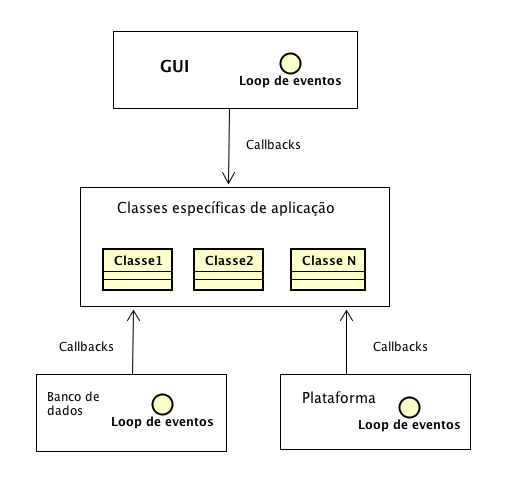
\includegraphics[scale=0.6]{fig/inversaodecontrole.png}
	\caption{Inversão de controle em \textit{framework}. (Adaptado de \cite{sommerville:2013})}
	\label{inversaodecontrole}
\end{figure}

O \textit{framework} ETL4NoSQL encaixa-se na categoria de aplicações corporativas, pois serve como base para aplicações de ETL, incorporando conhecimentos sobre a área de domínio para apoiar o desenvolvimento ao usuário final.




\subsection{Estudo Experimental de Software}

Esta pesquisa de dissertação considera a execução do estudo experimental de software para caracterizar, avaliar e propor melhorias ao framework ETL4NoSQL. O objetivo principal da aplicação do experimento é definir se o \textit{framework} proposto é uma ferramenta adequada para auxiliar no desenvolvimento de processos de ETL em dados estruturados, semi estruturados e não estruturados. Os participantes escolhidos foram as principais ferramentas de ETL encontradas na literatura. Os questionários utilizados para a coleta de dados são baseadas nos requisitos mínimos considerados pela literatura para ferramentas de ETL.

Segundo Travassos (2002), a experimentação é o centro do processo científico, por meio dos experimentos que é possível verificar teorias, explorar fatores críticos e formular novas teorias. O autor reforça ainda a necessidade de avaliar novas invenções e sugestões em comparação com as existentes.

Para Wohlin00, existem quatro métodos relevantes para experimentação em Engenharia de Software: científico, de engenharia, experimental e analítico. 

O paradigma indutivo, ou método científico, observa o mundo, pode ser utilizado quando se quer entender o processo, produto de software, ambiente. Ele mede e analisa, verifica as hipóteses do modelo ou teoria.  Já o método de engenharia observa as soluções existentes, é uma abordagem baseada na melhoria evolutiva, modifica modelos de processos ou produtos de softwares existentes com propósito de melhorar os objetos de estudo. O método experimental é uma abordagem baseada na melhoria revolucionária. Ela sugere um modelo, não necessariamente baseado em um existente, aplica o método qualitativo e/ou quantitativo, faz a experimentação, analisa e repete o processo. Por fim, o método analítico sugere uma teoria formal, é um método dedutivo que oferece uma base analítica para o desenvolvimento de modelos (Travassos, 2002).

Travassos (2002) sugere que a abordagem mais apropriada para a experimentação na área de Engenharia de Software seja o método experimental, pois considera a proposição e avaliação do modelo com os estudos experimentais.

Os principais objetivos relacionados à execução de um estudo experimental de software são: caracterização, avaliação, previsão, controle e melhoria a respeito de produtos, processos, recursos, modelos e teorias.

Os elementos principais do experimento são: as variáveis, os objetos, os participantes, o contexto do experimento, hipóteses e o tipo de projeto do experimento.

\section{Trabalhos Correlatos}

\noindent Esta seção apresenta os principais \textit{frameworks} correlatos a este trabalho encontrados na literatura, bem como os descreve  demonstrando suas características, seus pontos positivos e negativos.



\subsection{ARKTOS II}

O principal objetivo do ARKTOS II é facilitar a modelagem dos processos de ETL, de forma que o usuário define a fonte dos dados e o destino, os participantes e o fluxo de dados do processo. Como ilustrado na figura \ref{arktosii}, o usuário pode desenhar atributos e parâmetros, conectá-los ao seu esquema de dados, criar relacionamentos e desenhar arestas de um nó para outro de acordo com a arquitetura do grafo (\cite{vassiliadis:2005}).


\begin{figure}[h]
	\centering
	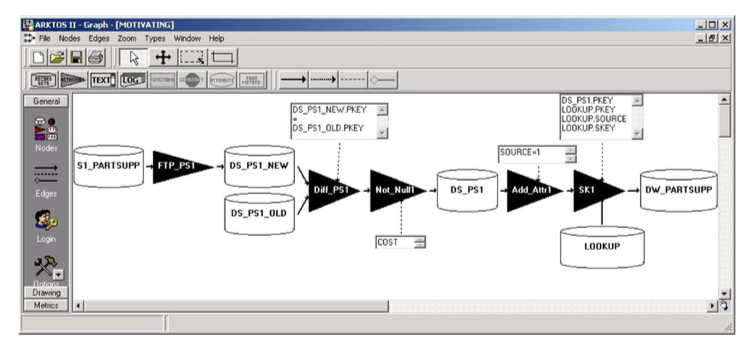
\includegraphics[scale=0.5]{fig/arktosii.png}
	\caption{Exemplo da Ferramenta ARKTOS II em uso (Adaptado de \cite{vassiliadis:2005})}
	\label{arktosii}
\end{figure}

A customização no ARKTOS II é oferecida pela reusabilidade de seus \textit{templates}. Os processos são armazenados em um repositório implementado em um banco de dados relacional. Os autores do ARKTOS II ainda pretendem melhorar a ferramenta permitindo mais formatos de dados como XML e orientado a objetos.


\subsection{PygramETL}

PygramETL é um \textit{framework} programável para desenvolvedores de ETL. Ele oferece a funcionalidade para desenvolver ETL demonstrando como deve-se iniciar um projeto. O propósito da ferramenta é facilitar a carga dos dados no DW gerenciado por banco de dados relacionais (RDBMS). Focando nos RDBMS como destino torna o desenvolvimento simples, não considerando outros tipos de estrutura de dados e a integração deles. Dessa forma, o PygramETL oferece suporte apenas a bancos de dados relacionais (\cite{thomsen:2009}).

\subsection{ETLMR}

ETLMR é um framework de ETL que utiliza \textit{MapReduce} para atingir escalabilidade. Ele suporta esquemas de DW como o esquema estrela, o \textit{snowflake}, e o \textit{slowly changing dimensions} \cite{liu:2011}. 

A figura \ref{etlmr} ilustra o fluxo de dados usando o ETLMR usando MapReduce. O processamento da dimensão é feito em uma tarefa do MapReduce, e o processamento do fato é feito por outra tarefa MapReduce. A tarefa MapReduce gera um número de tarefas map/reduce paralelas para processar a dimensão ou o fato. Cada tarefa consiste em inúmeros passos, incluindo a leitura dos dados no sistema de arquivos distribuído (DFS - distributed file system), execução da função de mapeamento, particionamento, combinação do mapeamento de saída, execução da função reduce e escrita dos resultados(\cite{liu:2011}).

\begin{figure}[h]
	\centering
	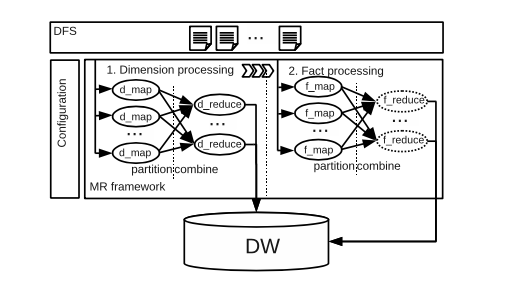
\includegraphics[scale=0.9]{fig/etlmr.png}
	\caption{Fluxo de dados ETL no framework MapReduce (Adaptado de \cite{liu:2011})}
	\label{etlmr}
\end{figure}

O ETLMR possui inúmeras contribuições, ele permite construir dimensões de ETL em alto nível processando os esquemas estrela, snowflake, SCDs e dimensões de dados intensivos. Pelo fato dele utilizar MapReduce, ele pode automaticamente processar mais de um nó enquanto ao mesmo tempo fornece a sincronização dos dados através dos nós. Além da escalabilidade, ele oferece alta tolerância à falhas, possui código aberto, e é fácil de usar com um único arquivo de configuração executando todos os parâmetros.

O principal objetivo do ETLMR é otimizar o tempo de processamento dos processos de ETL por meio do framework MapReduce. Porém, não há nada a respeito de como deve ser feita a modelagem dos processos de ETL.

\subsection{CloudETL}

O framework CloudETL é uma solução para processos de ETL que usa \textit{Hadoop} para paralelizar fluxos de ETL e \textit{Hive} para processar os dados de forma distribuída. Para o CloudETL o \textit{Hadoop} é a plataforma de execução dos processos de ETL e o \textit{Hive} é o sistema de armazenamento. Conforme a figura \ref{cloudetl}, os componentes do CloudETL são as APIs (interfaces de programação de aplicação), um conjunto de elementos para efetuar as transformações nos dados identificados como ETL \textit{transformers}, e um gerenciador de tarefas que controla a execução das tarefas submetidas ao \textit{Hadoop}. 

CloudETL fornece suporte de alto nível em ETL para construção de diferentes esquemas de DW, como esquema estrela, \textit{snowflake} e SCD (\textit{slowly changing dimensions}). Ele facilita a implementação de processos de ETL em paralelo e aumenta a produtividade do programador significativamente. Esta abordagem facilita as atualizações de SCDs em um ambiente distribuído \cite{liu:2013}.

\begin{figure}[h]
	\centering
	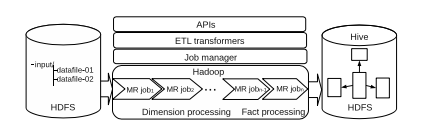
\includegraphics[scale=0.9]{fig/cloudetl.png}
	\caption{Arquitetura do CloudETL (Adaptado de \cite{liu:2013})}
	\label{cloudetl}
\end{figure}

O CloudETL é uma alternativa quando o problema é o processamento de um grande volume de dados por possuir a propriedade de processamento distribuído, porém não oferece nenhum suporte para modelagem de processos de ETL ficando a cargo do programador ou da equipe responsável pelo projeto de DW. 


\subsection{P-ETL}

P-ETL (Parallel - ETL) foi desenvolvido utilizando o \textit{framework} Hadoop com o paradigma MapReduce. Ele oferece duas maneiras de ser configurado: por meio de uma GUI (\textit{graphical user interface}) ou um arquivo de configuração XML. A figura \ref{petl} mostra a interface gráfica de configuração do P-ETL, ela é organizada em três abas: \textit{Extract, Transform, Load} e uma parte para parâmetros avançados. 

O processo de ETL do \textit{framework} inicia-se na aba \textit{Extract}, as configurações fornecidas pelas outras abas dependem desta primeira, principalmente o formato dos dados da fonte e sua estrutura. O primeiro passo da fase de extração é localizar a fonte de dados.  O arquivo base do P-ETL é no formato "csv" (\textit{Comma Separated Values}). Ele converte a fonte para o formato "csv" permitindo a entrada dos dados em vários formatos. Para acelerar a carga dos dados da fonte no HDFS (formato utilizado pelo \textit{Hadoop}), o P-ETL permite o usuário comprimi-los. A respeito da partição, o usuário pode escolher o tipo de partição (\textit{single, Round Robin, Round Robin by block}) e o número de dados por partição, além disso, ele pode configurar a extração pela quantidade de tuplas (por linhas ou blocos). A aba \textit{Transform} permite o usuário escolher um lista de funções para transformação, cada função deve ser especificamente configurada (condições, expressões, entradas, etc.), assim, as funções são executadas na ordem que foram inseridas. E finalmente, a aba \textit{Loading} permite configurar as tarefas de carga e incluir o destino dos dados (\textit{data warehouse, datamart, etc.}), os dados são comprimidos antes de serem carregados no HDFS e o separados no formato "csv" (\cite{bala:2014}).

\begin{figure}[h]
	\centering
	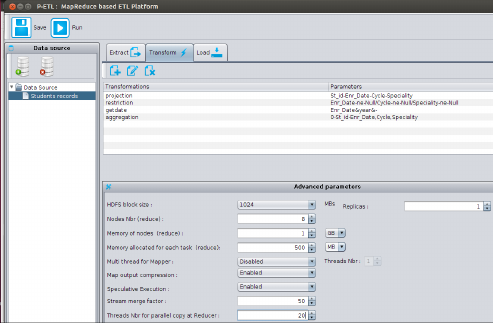
\includegraphics[scale=0.9]{fig/petl.png}
	\caption{Interface de configuração do P-ETL (Adaptado de \cite{bala:2014})}
	\label{petl}
\end{figure}

O P-ETL usa principalmente dois módulos do \textit{framework} Apache Hadoop: (i) HDFS para o armazenamento distribuído e a alta vazão para o acesso aos dados das aplicações, e (ii) MapReduce para processar paralelamente. Futuramente, o P-ETL pretende adicionar outras funções de transformação para realizar processos mais complexos, e oferecer um ambiente na nuvem, mais precisamente, virtualizar e transformá-lo numa arquitetura orientada à serviço (SOA - \textit{Service Oriented Architecture}) (\cite{bala:2014}).


\subsection{Big-ETL}

\cite{bala:2015} propõe em seu trabalho uma abordagem chamada Big-ETL, no qual define que funcionalidades de ETL podem ser executadas em \textit{cluster} utilizando o paradigma MapReduce (MR). O Big-ETL permite paralelizar e distribuir o processo de ETL em dois níveis: o processo de ETL (nível de granularidade maior), e a funcionalidade de ETL (nível de granularidade menor); dessa forma, melhorando o desempenho. Para testar a abordagem proposta, o autor utilizou o P-ETL com intuito de melhorar a ferramenta definindo o processo de ETL (nível de granularidade maior), e a funcionalidade de ETL (nível de granularidade menor) como níveis para o experimento, demonstrando ser uma boa alternativa para melhorar o desempenho nos processos de ETL.

Futuramente os autores pretendem apresentar um \textit{benchmark} no qual comparará quatro abordagens: processo de ETL centralizado; processo de ETL distribuído, Big-ETL e uma abordagem híbrida.

\subsection{FramETL}

O FramETL é um \textit{framework} para desenvolvimento de aplicações ETL. Ele oferece um ambiente programável e integrado para modelagem e execução de processos de ETL utilizando uma linguagem de programação. O autor utilizou conceitos de \textit{frameworks} como flexibilidade, extensibilidade, reuso e inversão de controle para o desenvolvimento do FramETL. Por meio desses conceitos, utilizando o \textit{framework}, o autor pode aplicar sua solução para construções de duas aplicações de ETL. Porém, \cite{silva:2012} não fez uso de BDs NoSQL, e o foco de sua ferramenta não era em dados \textit{Big Data}.

\subsection{Outras Ferramentas}

Esta seção apresenta outras ferramentas de ETL presentes no mercado e na literatura, mas que não possuem um foco em BDs NoSQL e \textit{Big Data}.
\subsubsection{Pentaho}

Pentaho Data Integration (conhecido também por \textit{\textbf{Kettle}}) é uma ferramenta \textit{open source} para aplicações de ETL. Ela é composta basicamente por quatro elementos: extração de diferentes fontes, transporte de dados, transformação dos dados e carga no \textit{data warehouse}. O \textit{Kettle} pode ser implementado em um único nó, bem como na nuvem, ou em \textit{cluster}. Ele pode carregar e processar \textit{big data} de várias formas oferecendo flexibilidade e segurança (\cite{mali:2015}, \cite{ETLtools}, \cite{pentaho}). Porém, por ser uma ferramenta genérica ela é de difícil customização. 

\subsubsection{Talend Studio}

\textit{Talend Open Studio} é uma plataforma de integração de dados que possibilita processos de integração, seu monitoramento e opera como um gerador de código, produzindo \textit{scripts} de transformação. Ele possui um repositório de metadados no qual fornece os dados (definições e configurações relacionados a cada tarefa) para todos os seus componentes. O Talend Studio é comumente utilizado para migração de dados, sincronização ou replicação das bases de dados  (\cite{mali:2015}, \cite{ETLtools}). 

\subsubsection{CloverETL}

\textit{Clover} é uma ferramenta ETL de código aberto considerada para transformação e integração, limpeza e distribuição de dados em aplicações, banco de dados e \textit{data warehouses}. Ela é baseada em Java e pode ser utilizada em linha de comando e é independente de plataforma  (\cite{mali:2015}).

\subsubsection{Oracle Data Integrator (ODI)}

\textit{Oracle Data Integrator} é uma plataforma de integração de dados que atende diversos requisitos de integração, desde grandes volumes de dados até o carregamento em \textit{batch}. As bases de dados de origem e destino podem incluir base de dados relacionais, arquivos XML, tabelas \textit{Hive, Hbase}, arquivos \textit{HDFS}, entre outros. Os usuários podem inserir filtros, junções, agregações, e outros componentes de transformação (\cite{silva:2016}). Porém, o ODI é uma ferramenta comercial e não permite a customização de suas aplicações.

\section{Considerações Finais}

Este capítulo discorreu a respeito das ferramentas de ETL encontradas na literatura. A maioria foca no desempenho ao lidar com \textit{Big Data}, nenhuma delas apresentou uma solução alternativa para modelagem de BDs NoSQL ficando a cargo do desenvolvedor encontrar meios para esquematizar os dados. A ferramenta P-ETL (\cite{bala:2014}) apresentou um arquivo "csv" como alternativa para obter diversos tipos de dados, porém não há um enfoque em BDs NoSQL. A abordagem PygramETL (\cite{thomsen:2009}) facilita a carga de dados, mas lida apenas com banco de dados relacionais. Para suportar processos de ETL em BDsNoSQL, propomos um \textit{framework} integrado, flexível e programável de ETL para BDs NoSQL que permite o uso do processamento distribuído/paralelo e a integração das diversas bases de dados existentes por se tratar de um \textit{framework} baseado em componentes.  